\chapter{Projektplan}
\section{Projektübersicht}
%TODO Text
\subsection{Zweck und Ziel}
%TODO Text
\subsection{Projektorganisation}
%TODO Tabelle
\section{Management Abläufe}
\subsection{Zeitbudget}
Der Projektstart ist am Montag, dem 20. Februar 2017. \\
Die Projektdauer beträgt 17 Wochen, und das Projektende ist am Freitag, dem 16. Juni 2017. \\

\noindent Während diesen 17 Wochen sind 360 Arbeitsstuden pro Projektmitglied eingeplant. Das entspricht pro Mitglied eine Arbeitszeit von ca. 22 Stunden pro Woche. Dies ergibt einen totalen Aufwand von ca. 720 Stunden.\\

\noindent Die wöchentliche Arbeitszeit von 22 Stunden kann bei Verzug oder bei unerwarteten Problemen auf maximal 30 Stunden erhöht werden. \\

\noindent Es sind gegenwärtig keine Absenzen während dieser Zeit geplant.

\subsubsection{Projektphasen}
Das Projekt wird in fünf Phasen unterteilt: Initialisierung, Analyse, Design, Realisierung und Abschluss.
\newline
\newline
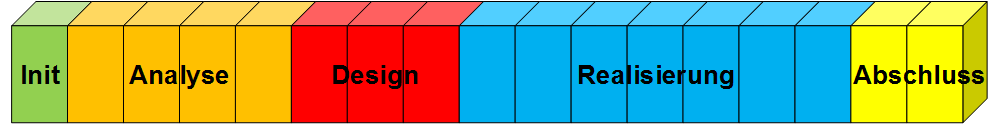
\includegraphics[width=1\textwidth]{images/phasen.png}
\newpage

\subsubsection{Meilensteine}
Das Projekt beinhaltet insgesamt fünf Meilensteine. \\

%TODO Tabelle

\subsubsection{Iterationen}
Die Dauer eines Iterationszyklus beträgt jeweils eine Woche. 
%TODO Tabelle

\begin{landscape}
\subsubsection{Arbeitspakete (Tickets)}
%TODO Tabelle
\end{landscape}


\subsection{Teammeetings}
Besprechungen finden wöchentlich jeweils am Montag statt. 
Eine Besprechung dauert in der Regel 30 Minuten und findet an der HSR statt. Bei einer Besprechung wird das weitere Vorgehen, sowie durchgeführte Arbeiten, fällige Arbeiten und auftretende Probleme besprochen. Weiter werden Arbeitspakete verteilt, damit beide Projektmitglieder wissen was zu tun ist. 

\subsubsection{Meeting mit Betreuern}
Die Meetings mit den Betreuern finden jeden Freitag um 14:00 Uhr statt. 
Die Meetings werden mit den Betreuern Beat Stettler und Urs Baumann in ihrem Büro durchgeführt. Die Dauer eines Meetings ist unterschiedlich und kann stark variieren. 

\section{Qualitätsmassnahmen}
\subsection{Versionierung}
Wie die Dokumentation wird auch der Sourcecode mit git versioniert und auf GitHub abgelegt. Es wird darauf geachtet, möglichst häufig auf den Stamm zu commiten.
\subsection{Reviews}
Regelmässige Reviews sind in einem iterativen Vorgehen unerlässlich. Die getätigte Arbeit muss ständig abgeglichen und in Frage gestellt werden. Aus Kosten-Nutzen Sicht sind Reviews das effektivste Mittel um die geforderte Qualität zu erreichen.\\ 

\noindent In diesem Projekt werden drei verschiedene Arten von Reviews durchgeführt. Zum einen sind dies regelmässige Code Reviews, zum anderen sind dies Requirement- und Architekturreviews.\\

\noindent Bei den regelmässigen Code Reviews wird besonders auf die gewählten Namen (Packages, Klassen, Methoden, Variablen), die Verständlichkeit vom Code und Code Smells geachtet.\\

\noindent Bei den Requirement Reviews wird sichergestellt, dass man den Wuenschen des Auftraggebers entsprechend entwickelt. Die Frage nach dem ''Was'' wird erneut gestellt und somit sichergestellt, dass man beim Projektende nicht ein qualitativ hochwertiges Produkt entwickelt hat, welches aber nicht die Wünsche des Auftraggebers abdeckt.\\ 

\noindent Beim Architektur Review wird besonders auf die nicht-funktionalen Anforderungen (NFA) geachtet. Diese wirken sich in den meisten Fällen auf die gewählte Architektur aus. Die gewählte Architektur muss mit den NFA's verträglich sein. Wenn zu spät im Projekt bemerkt wird, dass die Architektur geändert werden muss, kann dies sehr aufwändig sein.
\subsection{Code Metriken}
Code Metriken zeigen mögliche Fehler oder Schwachstellen im entwickelten Code auf. Es wird grundsätzlich zwischen statischen- und dynamischen Metrik Tools unterschieden. Bei den dynamischen Metrik Tools wird der Code ausgeführt. Beispiele wären Unit Tests und die dazugehörige Coverage. Bei den statischen Analysetools wird der Code nicht ausgeführt. Ein Beispiel wäre Checkstyle. Dieses Tool überprüft vor allem die Einhaltung von Style Richtlinien.\\

\noindent Um diese mächtigen Tools effektiv nutzen zu können, müssen sie in den Build Prozess mit eingebunden werden. SonarQube stellt ein Modul für Build-Management-Tools bereit, sodass statische Code Analysen automatisch beim Build ausgeführt werden.